\section{\imperia}
    \label{section:Imperia}
    % TODO: Wie werden Medien gespeichert?
    {\imperia} ist ein kommerzielles Enterprise Content Management und
    Web Content Management System, welches seit 1995 entwickelt
    \cite{imperia:about, imperia:historie} und von 
    der {\fernUni} zur Pflege ihrer Webseiten genutzt wird
    \cite{fernUni:imperia}.

    Dieses Kapitel geht auf die wichtigsten Merkmale und Konzepte
    dieses \gls{cms} ein.

    \subsection{Statische Generierung}
        \label{section:imperiaStaticGeneration}
        {\imperia} ist ein statisch generierendes \gls{cms}.
        Das bedeutet, dass es Inhalte basierend auf Vorlagen
        in Dateien generiert, die dann auf ein Zielsystem übertragen
        und dort beliebig und vor allem unabhängig von
        {\imperia} genutzt werden können
        \cite[Kapitel 1.1]{imperia:ecmd}.

        Die Generierung der Dateien und deren Übertragung auf ein Zielsystem
        werden zusammengefasst als "`Publizierung"' bezeichnet.

        % TODO Vorteile

    \subsection{Dokumente}
        \label{section:imperiaDocuments}
        Die zentrale Datenstruktur in {\imperia} sind Dokumente,
        da sie zur Speicherung von Inhalten dienen
        \cite[Kapitel 1.1]{imperia:ecmd}.
        Dokumente werden beim Anlegen stets einer Kategorie zugewiesen,
        die festlegt auf welcher Vorlage\footnote{vgl. Kapitel \ref{section:imperiaTemplates}}
        das Dokument basiert.
        Die Vorlage bestimmt wiederum welches Eingabeformular
        {\editors} zur Pflege der Inhalte des Dokumentes verwenden
        \cite[Kapitel 1.1.4]{imperia:ecmd}.
        
        {\imperia} speichert ein Dokument als simple Menge von
        Schlüssel-Wert-Paaren in einer relationalen Datenbank.
        Als Schlüssel -- auch Metavariablen genannt -- dienen die Namen der Felder des Eingabeformulars.
        Entsprechend übernimmt {\imperia} die Inhalte dieser Felder
        als Werte der Schlüssel-Wert-Paare.
        Diese allgemeine Datenstruktur ermöglicht die Nutzung der Inhalte
        in verschiedenen Ausgabeformaten, wie \gls{html}, XML, etc
        \cite[Kapitel 1.1.2]{imperia:ecmd}.

    \subsection{Vorlagen}
        \label{section:imperiaTemplates}
        Ein wichtiges Ziel von {\imperia} ist die Trennung von Inhalt
        und Layout einer Webseite.
        Zu diesem Zweck speichert es Inhalte layoutunabhängig
        in Dokumenten\footnote{vgl. Kapitel \ref{section:imperiaDocuments}}.

        Das Layout hingegen wird auf dem Dateisystem in Vorlagen festgehalten,
        die zwei Ziele verfolgen
        \cite[Kapitel 36]{imperia:ecmd}:

        \begin{enumerate}
            \item {\editors}n ohne technische Kenntnisse eine einfache Pflege von Inhalten zu ermöglichen
            \item Inhalte in das Layout zu integrieren
        \end{enumerate}

        Zur Erfüllung des ersten Zieles kann jede Vorlage ein Eingabeformular
        und dessen Felder spezifizieren.
        Dazu stehen geläufige Komponenten wie Textfelder,
        aber auch {\imperia} eigene Elemente zur Verfügung
        \cite[Kapitel 1.1.4]{imperia:ecmd}.
        Jeder Kategorie wird eine Vorlage zugewiesen,
        wobei eine Vorlage von mehreren Kategorien genutzt werden kann.
        Durch die Einteilung der Dokumente in Kategorien
        \footnote{vgl. Kapitel \ref{section:imperiaDocuments}}
        kann jedes Dokument somit einer Vorlage zugeordnet werden.
        Das durch diese Vorlage definierte Eingabeformular
        wird {\editors n} zur Pflege der Inhalte des Dokumentes präsentiert
        \cite[Kapitel 1.1.4]{imperia:ecmd}.

        Das zweite Ziel erreichen Vorlagen,
        indem sie neben dem Eingabeformular auch ein Gerüst für das
        Layout definieren.
        Über eine spezielle Syntax können sie an beliebigen Positionen
        Metavariablen\footnote{vgl. Kapitel \ref{section:imperiaDocuments}} referenzieren,
        deren Werte im Ausgabedokument an der entsprechenden Stelle integriert werden
        \cite[Kapitel 36]{imperia:ecmd}.

        Vorlagen können in zwei Varianten vorliegen.
        Die erste vereint sowohl die Definition des Eingabeformulares
        als auch die des Layouts in einer Datei.
        Ein {\editor} kann Dokumente dadurch nach dem Prinzip \gls{wysiwyg} bearbeiten.
        Die Eingabefelder entfernt {\imperia} automatisch im Ausgabedokument.
        Die zweite Variante trennt beide Definitionen in unterschiedliche Dateien.
        Dieses Vorgehen ist sinnvoll, wenn die Inhalte eines Dokumentes mit
        verschiedenen Layouts genutzt werden sollen.
        In diesem Fall existiert also eine Vorlage,
        die das neutrale Eingabeformular bestimmt
        und mehrere Layout-Vorlagen, die dieselben Inhalte unterschiedlich darstellen
        \cite[Kapitel 36]{imperia:ecmd}.

    \subsection{Workflows}
        Ein Dokument durchläuft von seiner Generierung bis zur
        Publizierung mehrere Verarbeitungsschritte,
        die in {\imperia} sogenannte Workflows festlegen.
        Jeder Kategorie wird dazu ein Workflow zugewiesen,
        den die Dokumente durchlaufen müssen.
        Ein solcher Workflow legt unter anderem fest,
        welche Schritte in welcher Reihenfolge
        zu durchlaufen sind
        \cite[Kapitel 1.1.5]{imperia:ecmd}.

        Ein typischer Workflow ist der Folgende
        \cite[Kapitel 1.1]{imperia:ecmd}:

        \begin{enumerate}
            \item Erstellung des Dokumentes und Angabe allgemeiner Daten
            \item Inhaltliche Pflege des Dokumentes
            \item Prüfung der Inhalte durch einen zweiten berechtigten \editor
            \item Publizierung der Inhalte
        \end{enumerate}

    \subsection{Architektur}
        \label{section:imperiaArch}
        {\imperia} basiert auf einer mehrschichtigen Client-Server-Architektur,
        die in Abbildung \ref{image:imperiaArchitektur} dargestellt ist.

        \begin{figure}[htb]
            \centering
            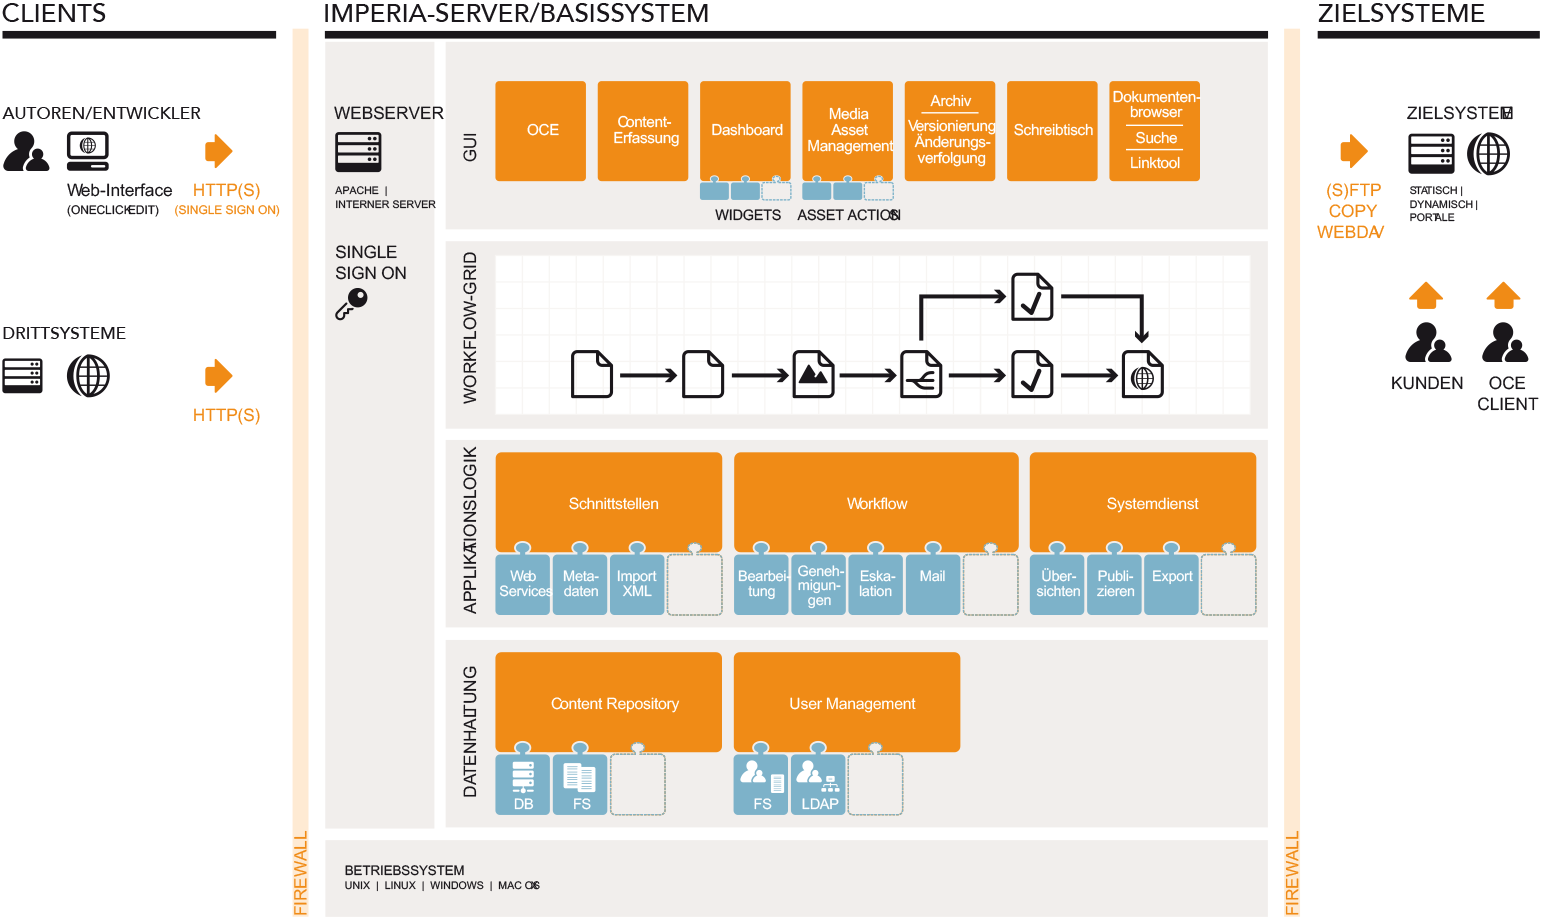
\includegraphics[width=\textwidth]{../resources/imperia/architektur.png}
            \caption{Architkektur von {\imperia} \cite{imperia:ecmd}}
            \label{image:imperiaArchitektur}
        \end{figure}

        Die wichtigste Komponente in dieser Architektur ist der imperia Server,
        der die zentralen Funktionen des Systems bereitstellt.
        Dazu gehören das Anlegen und Strukturieren von Projekten
        und Dokumenten sowie die Ausführung von Workflows.
        Nicht zuletzt verwaltet er die Datenhaltung.

        Die verschiedenen Nutzer des Systems wie {\editors} und Administratoren
        verwenden für ihre Arbeit eine Weboberfläche,
        die über HTTP(S) mit dem Server kommuniziert.
        Über das gleiche Protokoll können auch Drittsysteme den Server
        ansprechen und verschiedene Aktionen durchführen oder Daten abfragen.

        Sobald ein Dokument alle Workflow-Schritte durchlaufen hat,
        wird es durch eine automatische oder manuelle Publizierung
        in eine Datei generiert, die dann auf ein Zielsystem übertragen wird.
        Dieses System ist eigenständig und gehört nicht zu {\imperia}.
        Allerdings bietet es die Möglichkeit über Dienste wie (S)FTP
        die generierten Dateien zu empfangen.
        Ein Beispiel sind Webserver, auf die Webseiten publiziert werden,
        die sie dann Besuchern bereitstellen.